\part{肌肉驱动的运动}

\markboth{肌肉驱动的运动}{肌肉驱动的运动}


\chapter{肌肉驱动的模拟} \label{chap:chap10}


预测非常困难,
尤其是关于未来的预测。
\begin{flushright}
	——尼尔斯$ \cdot $玻尔
\end{flushright}


\begin{figure}[!htb]
	\centering
	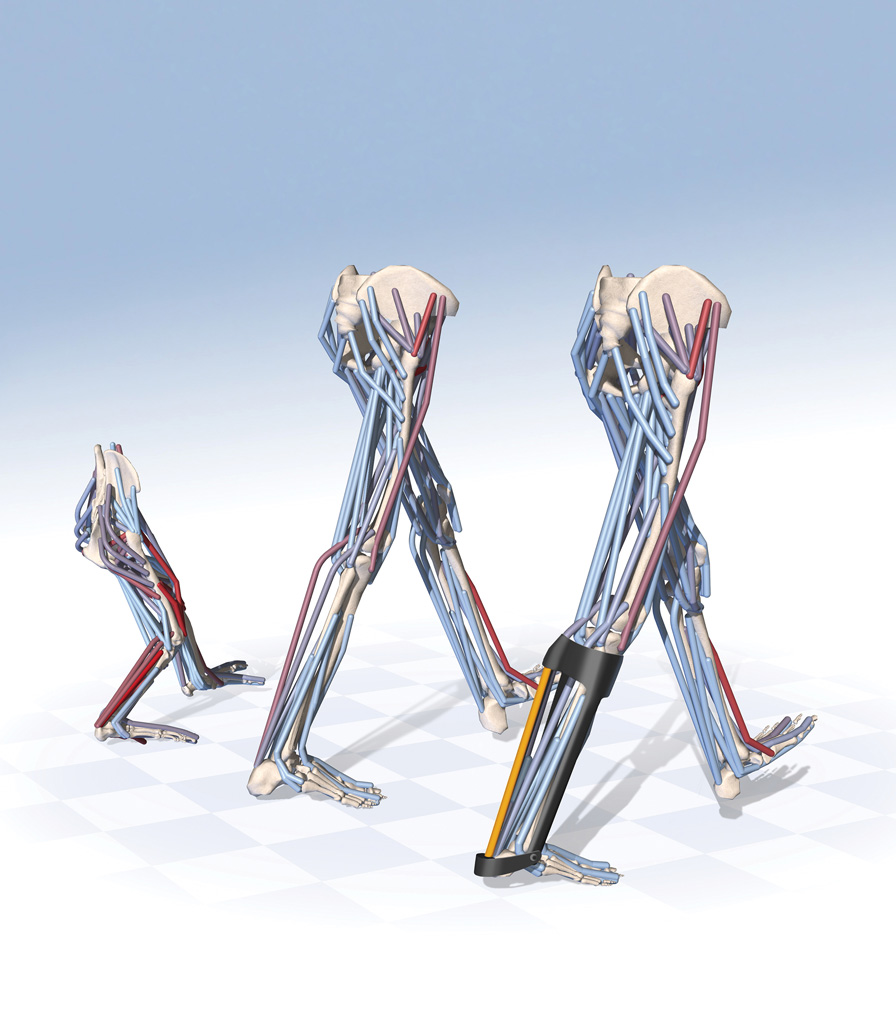
\includegraphics[width=0.9\linewidth]{chap10/10_0}
	% 加星号(*)表示不加编号
	\caption*{ \label{fig:10_0}}
\end{figure}

1983 年大学毕业后,我的第一份工作是帮助小公司编写计算机辅助设计软件。
当时我在科罗拉多州的一家计算机工厂工作,这家工厂刚刚生产出一台功能强大的新型图形计算机。
在当时,“强大”意味着它每秒可以在小屏幕上画几条线。
如果没有图形软件,没有人会使用我们的图形计算机,所以我的工作就是帮助其他公司的工程师将他们的计算机辅助设计软件在我们新推出的计算机上运行。
我逐渐意识到,几乎所有未来的产品都将在计算机上设计。
在我申请研究生院的时候,我提议开发用于手术设计的计算机图形工具。


2 年后,我进入研究生院,有幸加入了斯坦福大学设计组由费利克斯$\cdot$扎亚克领导的生物力学研究实验室。
扎亚克是一位热衷于理解运动控制的神经科学家,他几十年来一直在进行各种精妙的实验,测量跳跃等动作中的肌肉激活模式、地面反作用力以及关节运动。
他意识到,要将这些实验数据整合起来,全面理解运动过程中的肌肉功能,仅仅依靠专业的数据分析是不够的。


仅靠实验测量不足以了解运动过程中的肌肉动作,原因有二。
首先,像肌肉产生的力量这样重要的量通常无法在实验中测量。
其次,仅通过实验观察很难建立因果关系。
例如,可以在行走过程中测量地面反作用力(第~\ref{chap:chap2}~章),并将其用于估计身体重心的加速度。
然而,单靠地面反作用力测量几乎无法了解肌肉如何影响身体重心的加速度,从而无法了解肌肉如何影响行走过程中支撑身体重量和推动身体向前的关键任务。
可以分析肌电图信号(第~\ref{chap:chap4}~章)来了解肌肉何时活跃,但不能揭示哪些身体运动是由每块肌肉的活动引起的。


我们需要一个新的框架来推进我们对运动过程中肌肉功能的理解。
这个框架必须揭示肌肉激活、肌肉力量、地面反作用力和身体运动之间的关系。


肌肉驱动的运动模拟提供了这一框架。
模拟可以估算肌肉力量,并揭示因果关系,例如行走过程中肌肉对地面反作用力的贡献。
我们还可以利用模拟来预测身体对疾病、手术或肌肉激活改变的反应。
这些能力使我们能够表征运动过程中肌肉的动作,并设计手术和辅助设备。


1985 年,当我加入扎亚克的研究小组时,他和他的学生们正处于开发肌肉驱动模拟的前沿。
加入这个小组后,我开启了一段持续 30 多年的旅程,专注于创建肌肉驱动模拟并进行分析,以改善生物力学受损人群的运动能力。
大学毕业后,我从事的工作在两年内就开发出了用于工程产品的计算机辅助设计工具,而开发用于理解人体运动复杂性的计算机辅助设计工具却成了我毕生的挑战。


本章介绍了我在创建肌肉驱动模拟方面的一些经验。
本章首先阐述了为什么在没有模拟的情况下很难确定运动过程中肌肉的动作,以及为什么文献中充斥着关于肌肉功能的错误结论。
接下来,我们将讨论构建和分析肌肉驱动模拟以正确确定肌肉动作的 4 个阶段。
然后,本章介绍了我和同事开发的开源模拟软件,该软件旨在促进全球合作,让成千上万的研究人员能够构建和共享运动的计算机模拟。
我的目标是通过齐心协力推动这一领域的发展。


\section{理解运动过程中的肌肉动作是一项挑战}

基于肌肉几何形状、肌电图测量和观察到的运动来推断其动作的实验方法无法正确解释肌肉如何驱动身体。
仅基于解剖学知识的分析常常会导致关于肌肉功能的错误结论。
例如,许多解剖学和生物力学文献将比目鱼肌描述为使踝关节跖屈的肌肉。
比目鱼肌确实会产生踝关节跖屈力矩,从而确实使踝关节跖屈,但该肌肉也能执行其他动作(图~\ref{fig:10_1})。
这些动作源于一种称为动态耦合的效应。

\begin{figure}[!htb]
	\centering
	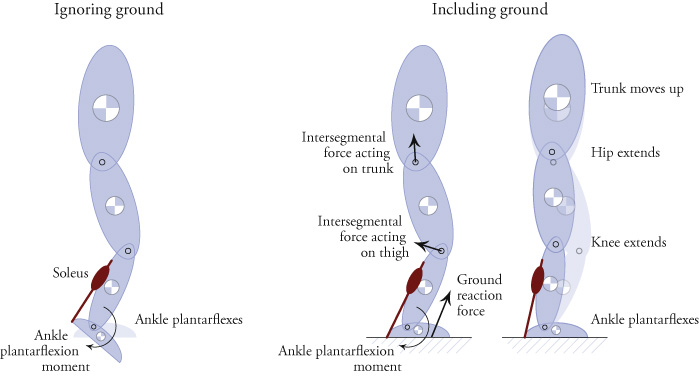
\includegraphics[width=1.0\linewidth]{chap10/10_1}
	\caption{单肢站立时比目鱼肌的动作,忽略(左)动态效应和考虑(右)动态效应。
		比目鱼肌跖屈产生的踝关节跖屈力矩在两种情况下都会使踝关节跖屈,但当考虑地面反作用力时,由于动态耦合作用,该力矩还会影响其他关节和身体部位\cite{anderson2006simulation}。 \label{fig:10_1}}
\end{figure}


动态耦合描述了一个身体节段的运动由于诱导力而影响另一个节段运动的现象。
如图~\ref{fig:10_1}~所示,比目鱼肌产生的力不仅会产生踝关节跖屈力矩,还会诱导全身节段间的力和关节加速度。
这些节段间的力的大小和方向取决于肌肉施加的力、肌肉的力臂、身体节段的质量和惯性以及身体的姿势。
在图~\ref{fig:10_1}~右侧的示例中,比目鱼肌产生的力使小腿产生逆时针的角加速度,这需要膝关节向上和向左加速。
大腿及其相邻节段的惯性抵抗了这种加速度,并在膝盖处产生节段间的力,这反过来又加速大腿,依此类推。
因此,尽管比目鱼肌只跨越踝关节,但它却加速了身体的所有关节。


在许多情况下,动态耦合产生的节段间力足够大,从而影响我们对肌肉动作的解读。
虽然远离肌肉的关节处的“肌肉诱导”加速度通常较小,但在附近关节处却可能很大。
例如,已证明,在站立时,比目鱼肌使膝关节伸展的加速度甚至大于使踝关节跖屈的加速度\cite{zajac1989determining}。
此外,他们还指出,双关节肌肉可以诱导与它穿过的其中一个关节产生的力矩相反的关节加速度。
例如,虽然腓肠肌产生膝关节屈曲力矩和踝关节跖屈力矩,但它仍然可以诱导膝关节伸展加速度或踝关节背屈加速度(图~\ref{fig:10_2})。
这些看似不协调的加速度在腓肠肌激活时是可能的,因为例如,它产生的膝关节屈曲力矩引起的膝关节屈曲加速度可能会被它产生的踝关节跖屈力矩引起的膝关节伸展加速度所掩盖。
许多生物力学研究在解释肌肉动作时忽略了动态耦合,并得出了错误的结论。
对于由数十个身体节段、关节和肌肉组成的肌肉骨骼系统来说,推断运动过程中肌肉的动作是一项挑战。
需要肌肉驱动的模拟来应对这一挑战。


\begin{figure}[!htb]
	\centering
	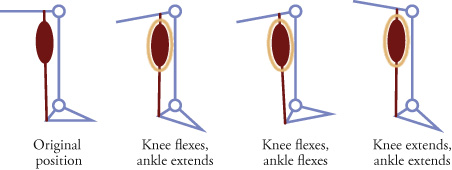
\includegraphics[width=0.75\linewidth]{chap10/10_2}
	\caption{双关节肌肉可以诱导关节加速度,该加速度与其在与其交叉的某个关节上产生的力矩相反。
		例如,从图中所示的初始位置(最左侧),腓肠肌产生的力可能会使膝关节和踝关节屈曲或伸展,如图所示,这是由于动态耦合作用\cite{zajac1993muscle}。 \label{fig:10_2}}
\end{figure}


你可能想知道肌肉是否真的会产生与施加力矩方向相反的加速度。
我以前也曾怀疑过。
史蒂夫$\cdot$皮亚扎是我实验室的一名学生,他创建了肌肉驱动的行走摆动阶段模拟(Piazza and Delp, 1996)。
他的模拟表明,在某些情况下,腘绳肌会产生髋屈曲加速度。
回想一下,腘绳肌在髋后交叉,因此,许多科学家认为这些肌肉总是会产生髋关节伸展。
运动方程分析证实了髋屈曲确实可能产生,但我们的临床同事对此表示怀疑。
尤其是杰奎琳$\cdot$佩里,一位世界领先的肌肉和步态专家,也是我的科学偶像之一,她不相信我们的结果,想要更多证据。
因此,史蒂夫制造了“说服器”,这是一种简单的装置,类似于一条腿,在腘绳肌所在的位置有一根金属丝。
当我们在适当的条件下拉动腘绳肌的金属丝时,髋关节会轻微弯曲。
史蒂夫和我都深信不疑,我们的临床同事,包括佩里博士,也深信不疑。


\section{创建肌肉驱动的模拟}

牛顿运动定律的方程表征了人体的动力学。
我们可以通过求解这些方程来预测人体的运动方式,这个过程被称为动态模拟。
“肌肉驱动”的动态模拟可以预测肌肉产生的力量在行走和跑步等运动过程中如何影响身体各个部位的运动。


开发、测试和分析肌肉驱动模拟的过程包括 4 个阶段(图~\ref{fig:10_3})。
在第 1 阶段,您将创建一个计算模型,该模型能够以足够的精度描述肌肉骨骼系统的动态行为,以回答您的研究问题。
如果其他人已经创建并分享了适合您研究的模型,您可以跳过这个繁琐的步骤。
第 2 阶段涉及计算一组肌肉激励,当将这些激励应用于模型时,会生成感兴趣运动的模拟。
第 3 阶段通过将模拟结果与实验测量结果进行比较,确认模拟充分代表了感兴趣的运动。
在第 4 阶段,您将分析模拟以回答您的研究问题。
我们将在接下来的章节中探讨每个阶段。


\begin{figure}[!htb]
	\centering
	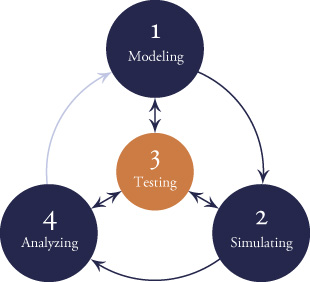
\includegraphics[width=0.5\linewidth]{chap10/10_3}
	\caption{创建和分析肌肉驱动模拟的过程包括
		(1)\textit{建模}肌肉骨骼动力学,
		(2)\textit{模拟}运动,
		(3)\textit{测试}模拟的准确性,以及
		(4)\textit{分析}模拟以回答特定的研究问题。 \label{fig:10_3}}
\end{figure}


\section{第一阶段:肌肉骨骼系统动力学建模}

肌肉骨骼动力学模型使我们能够计算由每种肌肉力量引起的运动。
我们四阶段流程的第一阶段是使用描述肌肉激活动力学、肌肉肌腱收缩动力学、肌肉骨骼几何结构和骨骼动力学的方程(图~\ref{fig:10_4})来创建肌肉骨骼系统模型。
这些方程表征了肌肉骨骼系统响应肌肉刺激时的时间依赖性行为。

% 和1_12.pdf一样
\begin{figure}[!htb]
	\centering
	\includegraphics[width=1.0\linewidth]{chap1/1_12}
	\caption{肌肉驱动模拟的要素。
		来自神经控制器的\textit{激励}通过肌肉激活和收缩动力学模型产生肌肉激活和肌肉力量。
		这些力量传递到骨骼,产生关节\textit{力矩},从而加速身体各节段的运动。
		\textit{感觉反馈}会修改神经指令。
		反馈还表明身体运动会影响系统的其他元素。 \label{fig:10_4}}
\end{figure}

正如我们在第~\ref{chap:chap4}~章中看到的,肌肉兴奋和激活之间的关系受运动单元动作电位和横桥循环的动态控制。
肌肉的激活 ($a$) 可以通过将其时间导数 ($\dot{a}$) 与电流激活和兴奋 ($u$) 关联来建模,如公式~\ref{eq:4_1}~所示。


肌肉激活是肌肉-肌腱收缩动力学模型的输入,肌肉-肌腱执行器(和)的长度和伸长速度也是如此。
如第~\ref{chap:chap5}~章所述,肌肉和肌腱的动力学受横桥形成的时间过程、肌动蛋白丝的滑动以及肌腱的动力学控制。
肌肉产生的力量 ($F^M$) 并通过其肌腱传递的力量 ($F^T$) 可以用四条无量纲曲线和五个肌肉特定参数来估算,如第~\ref{chap:chap5}~章所述。
当应用于骨骼时,肌肉力量会产生关于关节的力矩,如第~\ref{chap:chap6}~章所述。
肌肉产生的关节力矩导致关节和身体节段加速,从而产生运动。


可以使用身体运动方程来计算身体对肌肉力量和其他负荷的响应加速度:
\begin{equation}
	\underline{\ddot{q}} = M^{-1} (\underline{q})
			\{
				\underline{F}^G (\underline{q}) + 
				\underline{F}^C (q, \dot{q}) + 
				R(\underline{q}) \underline{F}^T (\underline{u}) + 
				\underline{F}^E (\underline{q}, \underline{\dot{q}})
			\}  \label{eq:10_1}
\end{equation}
%
在这组方程中,$\underline{q}$ 、$\underline{\dot{q}}$和 $\underline{\ddot{q}}$ 分别是关节的位置、速度和加速度。
$M^{-1} (\underline{q})$是系统质量矩阵的逆,其中包含身体各节段的质量和惯性特性。
如公式~\ref{eq:10_1}~所示,质量矩阵定义了力和关节加速度之间的关系。 
$\underline{F}^G (q)$是由重力引起的力的矢量。
$\underline{F}^C (\underline{q}, \underline{\dot{q}})$ 是科里奥利力和离心力的矢量,这些力是在牛顿运动定律应用于固定在旋转物体上的参考系时产生的。
$R(\underline{q})$是肌肉力臂矩阵, $\underline{F}^T (u)$是肌腱力的矢量,它是肌肉激励的函数($\underline{u}$)。
肌肉力臂决定了肌腱力施加到骨骼上时产生的关节力矩。
最后,$\underline{F}^E (q, \dot{q})$是外力的矢量,用于表征身体与其环境(例如地面反作用力)之间的相互作用。
分析公式~\ref{eq:10_1}~使我们能够计算每块肌肉力引起的加速度,从而确定复杂多关节系统中肌肉的动作。


图~\ref{fig:10_4}~所示的建模方法已用于创建各种运动的肌肉驱动模拟。
一些研究使用相对简单的肌肉骨骼系统模型。
例如,仅包含少量自由度且仅由少量肌肉驱动的二维模型可能足以捕捉感兴趣的现象(图~\ref{fig:10_5})。
在其他情况下,可能需要具有多个自由度和数十块肌肉的三维模型来阐明单个肌肉对观察到的运动的贡献(图~\ref{fig:10_6})。
需要注意的是,模型的实用性并不总是随着模型复杂度的增加而提高。
事实上,使用比回答研究问题所需更复杂的模型会适得其反。
额外的复杂性会增加构建和验证模型、生成模拟以及分析模拟结果所需的工作量。
因此,请注意:复杂性会导致困惑!


\begin{figure}[!htb]
	\centering
	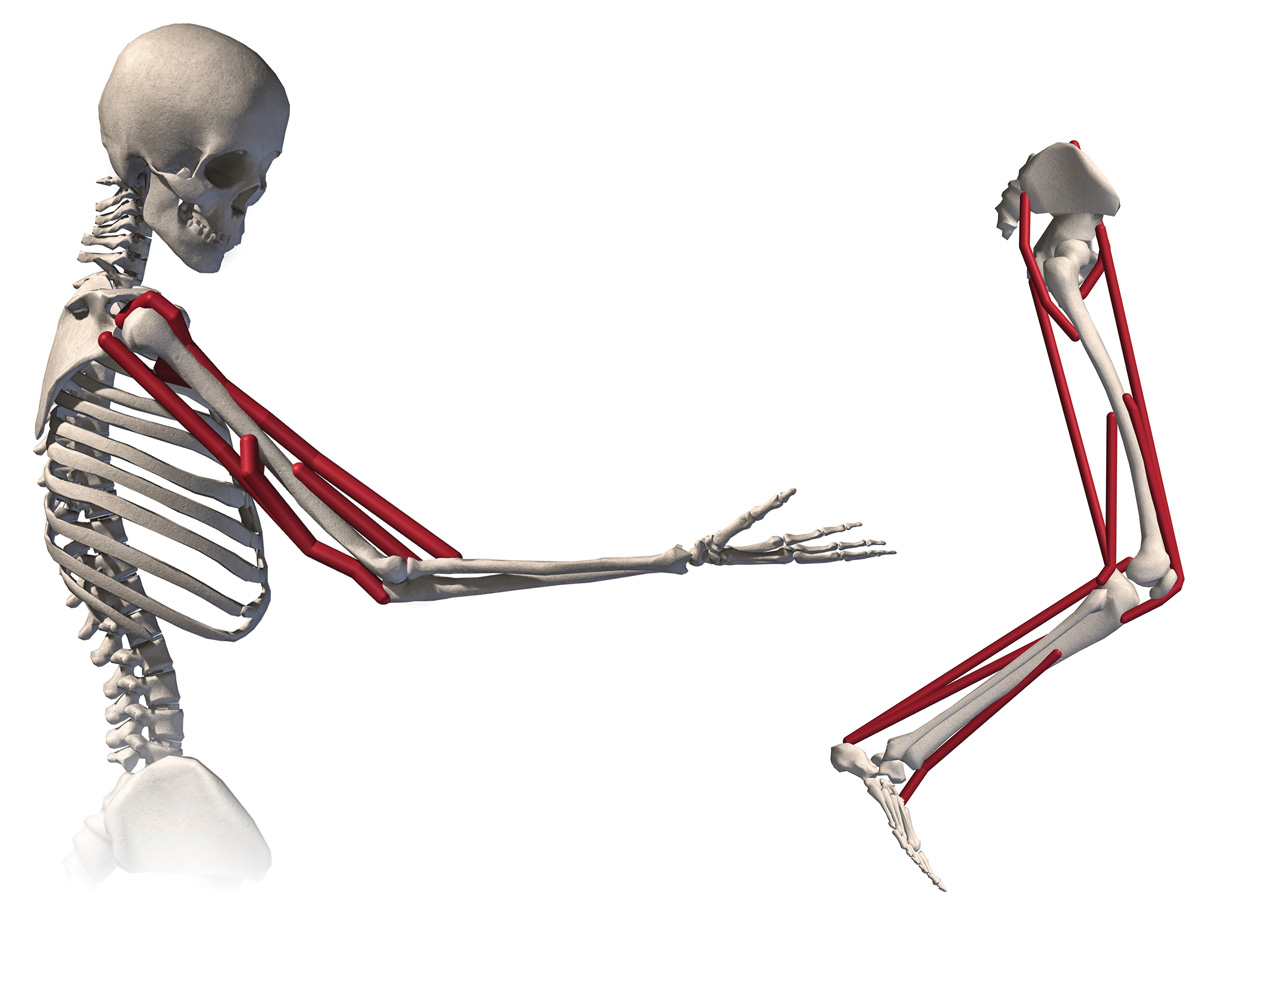
\includegraphics[width=1.0\linewidth]{chap10/10_5}
	\caption{用于生成肌肉驱动模拟的上肢和下肢平面肌肉骨骼模型。
		此类简单模型可能足以研究平面肘部屈曲或步态过程中腿部摆动的动力学\cite{murray1995variation,delp1990interactive}。\label{fig:10_5}}
\end{figure}


\begin{figure}[!htb]
	\centering
	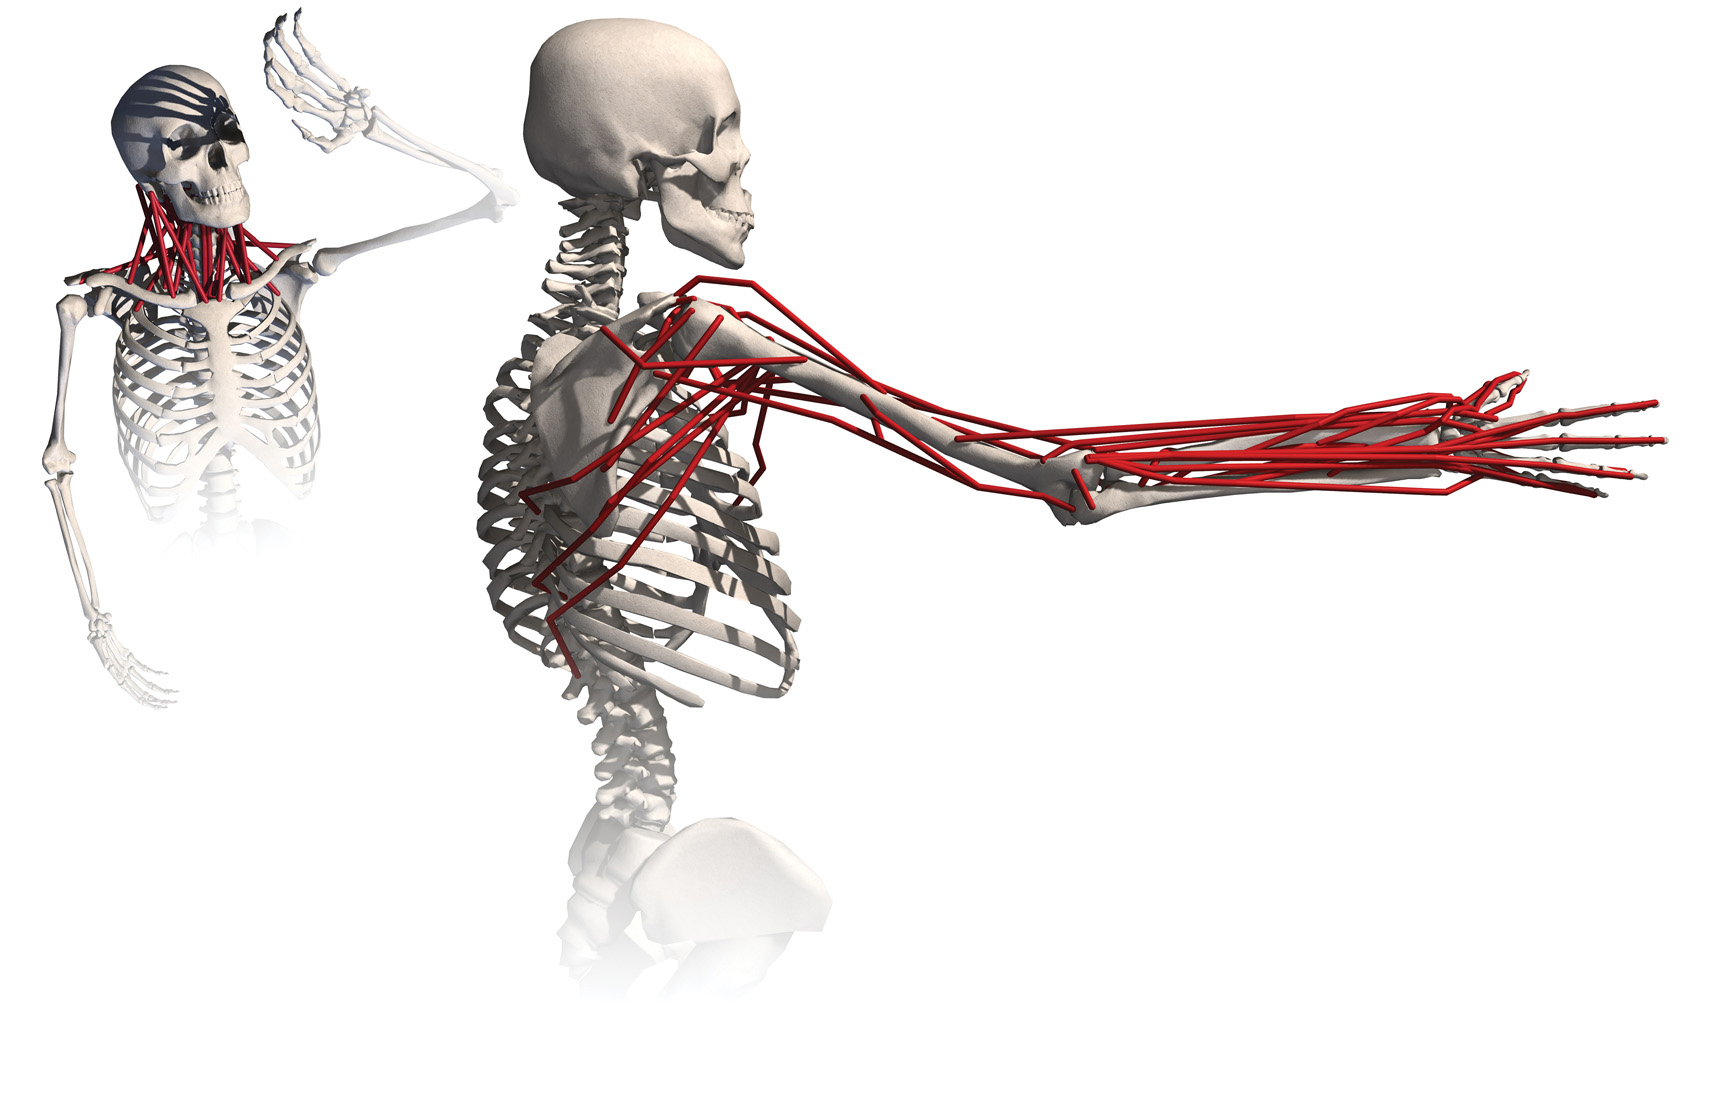
\includegraphics[width=1.0\linewidth]{chap10/10_6}
	\caption{详细的颈部和上肢肌肉骨骼模型,用于生成肌肉驱动的颈部损伤和伸手任务模拟。
		这类相对复杂的模型可以提供有关单个肌肉活动、力量产生和能量学的详细信息\cite{vasavada1998influence,cazzola2017cervical,saul2015benchmarking}。 \label{fig:10_6}}
\end{figure}


一旦为特定研究选定了通用模型,就必须校准该模型,使其与每位研究参与者的几何形状和力量相匹配。
您可以根据运动捕捉实验(参见第~\ref{chap:chap7}~章)中的测量结果,调整每个身体部位的尺寸和惯性属性,从而校准模型。
模型关节的位置、方向和运动范围可以根据实验结果进行调整,实验中受试者会通过一系列标准动作移动每个关节。
肌肉的路径和其他参数可以通过临床检查、力量测试以及诸如跳高之类的活动进行校准。
校准模型的一种有效方法是通过优化来调整模型参数,从而最大限度地减少测量值与模拟值之间的误差。


虽然我们在这里只用了几页纸,但构建、校准和验证一个新的肌肉骨骼模型可能需要数年时间。
我敦促模型开发者与生物力学界分享他们的成果,以便其他人能够在此基础上进行进一步的开发。



\section{第二阶段:模拟运动}

为了生成运动模拟,需要对动态模型的微分方程进行时间上的数值积分。
如果模拟由肌肉驱动,则必须应用一组肌肉激励(例如公式~\ref{eq:10_1}~中的激励)。
这些肌肉激励通常由优化器生成。
此外,还必须提供模拟的初始条件,即每个状态变量在初始时刻的值。
状态变量包括关节角度和角速度、肌肉激活度、肌纤维长度以及其他随时间变化的量。
控制微分方程(公式~\ref{eq:10_1})描述了这些状态变量随其当前值变化的速率。
这些方程的数值解可以得出状态变量的轨迹,由此可以计算所有其他与状态相关的量,例如肌肉和肌腱力、肌腱应变、关节接触力以及每块肌肉消耗的代谢能量。


找到一组能够产生协调运动的肌肉激励是一项挑战,尤其是对于像行走这样复杂的运动。
不仅必须控制多个自由度,还必须考虑肌肉随时间变化的非线性力产生特性。
此外,我们通常希望生成与实验测量值相符的模拟结果,例如关节角度轨迹或随时间变化的代谢功率消耗。
为了克服这些挑战,可以使用动态优化(第~\ref{chap:chap9}~章)来找到能够最小化特定性能标准的肌肉激励。
肌肉激励可以通过多种方式参数化。
一种常见的方法是将每个激励信号表示为随时间均匀分布的点序列,其中某一时刻的激励是使用线性插值从两个相邻点计算得出的(图~\ref{fig:10_7})。
在这种情况下,优化器会通过调整每个点的高度来最大化性能。


\begin{figure}[!htb]
	\centering
	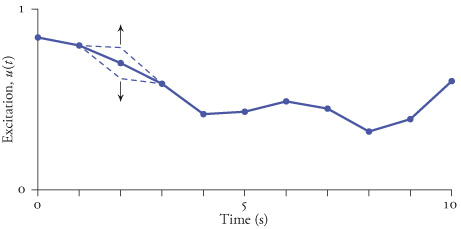
\includegraphics[width=0.8\linewidth]{chap10/10_7}
	\caption{表示肌肉兴奋的曲线可以参数化为随时间变化的点序列。
		优化器通过求解每块肌肉每个点的高度来预测运动过程中的肌肉协调性。 \label{fig:10_7}}
\end{figure}

两种优化策略可用于生成肌肉驱动的模拟。
一种方法是求解最优跟踪问题,其中目标函数反映模拟量与测量量(例如关节角度、关节力量和地面反作用力)之间的差异。
通过在模拟持续时间内最小化目标函数,模型将被驱动以重现实验观察到的运动。
例如,使用以下目标函数生成肌肉驱动的截肢步态模拟,以跟踪实验测量值\cite{silverman2012muscle}:
%
\begin{equation}
	J = \sum_{i} \sum_{j} \frac{(y_{ij} - \hat{y}_{ij})}{\sigma_i^2} \label{eq:10_2}
\end{equation}
%
其中 $y_{ij}$ 是变量 $i$(包括关节运动学和地面反作用力矢量的分量)在时间步 $j$ 的测量值,$\hat{j}_{ij}$是模拟中对应的量,$\sigma_i^2$是实验量 $y_i$ 的方差。
平方误差除以相应实验变量的方差,因此方差较大的变量跟踪精度较低。


解决最优跟踪问题可能耗费大量的计算资源。
即使是像跟踪单个步态周期的运动学这样的简单问题,也可能需要数小时甚至数天才能解决。
我有幸与 Darryl Thelen 和 Clay Anderson 合作,当时他们正在开发计算肌肉控制算法,该算法解决最优跟踪问题的速度比之前的方法(Thelen 等人,2003)快 100 到 1000 倍。
现在很多人都在使用这种方法。


生成肌肉驱动运动模拟的第二种方法是动态优化,其中使用诸如最小化总能量消耗或最大化运动表现指标之类的目标来生成运动。
正如我们在第九章中看到的,Carmichael Ong 及其同事使用一个目标函数生成了立定跳远的模拟,该函数奖励更长的距离并惩罚不良解决方案(例如那些可能导致受伤的解决方案)。
当时也在我的实验室工作的 Tim Dorn 使用类似形式的目标函数来生成负重行走和倾斜行走的肌肉驱动模拟:
%
\begin{equation}
	J = w_{\text{fall}} J_{\text{fall}} +
		w_{\text{speed}} J_{\text{speed}} + 
		w_{\text{head}} J_{\text{head}} + 
		w_{\text{effort}} J_{\text{effort}} \label{eq:10_3}
\end{equation}
%
其中,$J_{\text{fall}}$ 惩罚不稳定的步态,$J_{\text{speed}}$ 惩罚与目标速度不一致的步态,$J_{\text{head}}$ 惩罚涉及不切实际头部运动的步态,$J_{\text{effort}}$ 惩罚耗能较高的步态,权重 $w_i$ 平衡这些相互竞争的目标。
求解这个动态优化问题可以模拟各种场景下的行走,包括模拟人类负重上坡行走\cite{dorn2015predictive}。



\section{第三阶段:测试动态模拟的准确性}

开发出肌肉骨骼系统模型后,您必须确认该系统的行为能够以足够的精度再现,以解答您的研究问题。
这个过程被称为验证。
我的同事 Jennifer Hicks 带领团队撰写了一篇综述文章,探讨了所有参与计算机模拟的人都面临的问题:
我的模型足够好吗\cite{hicks2015my}?


所有模型的设计都基于预期用途,且存在局限性。
在选择研究模型时,务必注意这些局限性。
例如,必须确认某些假设的适用性,例如将短而硬的肌腱近似为刚性连接以提高模拟速度(图~\ref{fig:10_8})。
对于肌腱较短的肌肉,将肌腱表示为弹性结构会显著增加模拟肌肉-肌腱动力学所需的时间,且准确性不会显著提高。
然而,对于肌腱较长的肌肉,当假设肌腱为刚性时,肌纤维长度(以及肌肉力量)的误差会很大。
因此,我通常使用刚性肌腱模型来表示肌腱较短的肌肉,但当肌腱至少与肌纤维等长时,我会考虑肌腱的弹性特性。

\begin{figure}[!htb]
	\centering
	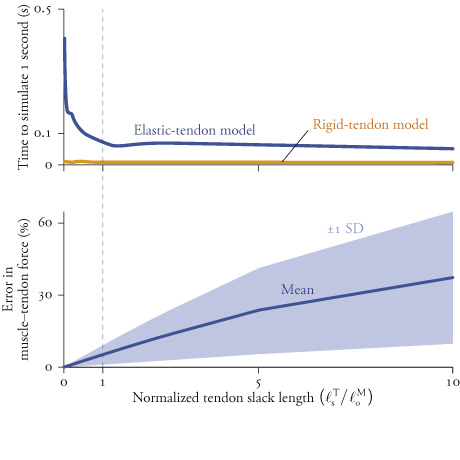
\includegraphics[width=0.77\linewidth]{chap10/10_8}
	\caption{刚性肌腱近似法可以大幅缩短模拟肌腱相对较短的肌肉所需的时间(上图),但会引入肌肉-肌腱力的误差(下图),尤其是在肌腱长度相对于最佳纤维长度较长的情况下\cite{millard2013flexing}。 \label{fig:10_8}}
\end{figure}

1990 年,我开发了一个膝盖模型,用简单的几何形状来表示复杂的生物接触面(图~\ref{fig:10_9})。
当时计算机速度慢且价格昂贵,所以我需要一个能够以较少的计算量计算出穿过膝盖的肌肉力臂的模型。
该模型在近 30 年的时间里一直表现良好。
然而,如果我需要一个模型来计算膝盖内的接触应力,我会使用更详细的关节接触面几何表示。
现在已经有了详细的生物关节模型,可以利用现有的计算资源。


\begin{figure}[!htb]
	\centering
	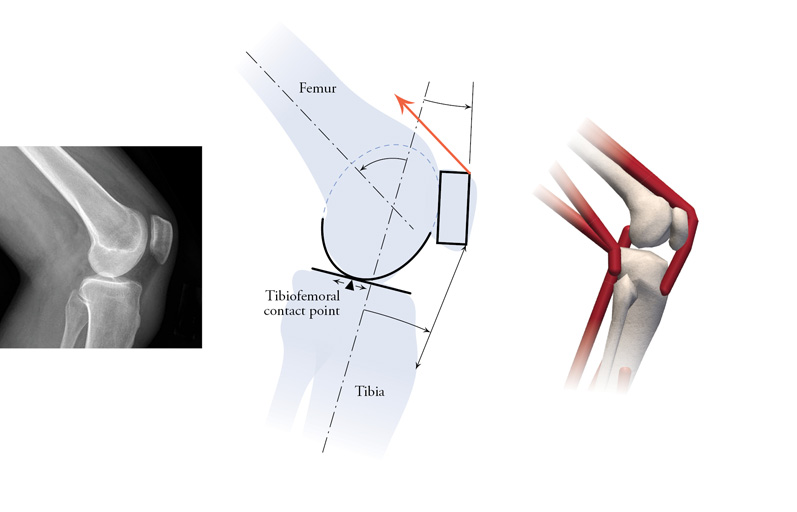
\includegraphics[width=1.0\linewidth]{chap10/10_9}
	\caption{在许多研究中,膝盖中复杂的生物接触面(左)可以用更简单的几何形状(中)来近似,并纳入肌肉骨骼模型(右)以提高模拟速度。 \label{fig:10_9}}
\end{figure}


我们通过将模拟预测的量与类似的实验测量值进行比较来测试模拟。
正如我们已经看到的,我们可以将肌肉驱动模拟中的关节角度、关节力矩​​、地面反作用力和肌肉激励模式与实验测量的运动学、动力学和肌电图数据进行比较。
例如,我们在第~\ref{chap:chap9}~章中概述的立定跳远模拟包括一个简单的脚与地面接触模型。
虽然该模型不能重现实验测量的地面反作用力的所有细节(图~\ref{fig:10_10}),但我们模拟的力随时间的积分与实验测量的地面反作用力的积分相似。
因为力的积分是跳跃距离的主要决定因素,所以我们认为简单的脚与地面接触模型已经足够好了。


\begin{figure}[!htb]
	\centering
	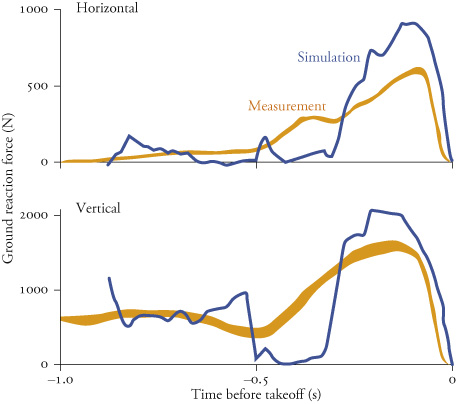
\includegraphics[width=0.9\linewidth]{chap10/10_10}
	\caption{立定跳远落地阶段的水平(上)和垂直(下)地面反作用力。
		使用动态优化生成的模拟结果(蓝色)与相应的实验数据(橙色;95\% 置信区间,3 位受试者每人 6 次跳跃\cite{ashby2002role})进行了比较\cite{ong2015simulation}。\label{fig:10_10}}
\end{figure}


最重要且最具挑战性的比较之一是模拟肌肉激活与实验记录的肌电图模式之间的比较。
这种比较很重要,因为肌肉激活的时间会影响对肌肉功能的解读。
这种比较很有挑战性,因为肌电图记录非常嘈杂,通常只收集一部分肌肉的数据。
在 Sam Hamner 分析他的跑步模拟之前,他将他模拟的激活模式与他在实验中收集的肌电图测量值进行了比较(图~\ref{fig:10_11})。
目前没有既定的标准来确定何时匹配足够好,所以 Sam 和我必须运用我们的最佳判断来决定如何解释与他的模拟激活相关的不确定性。
一旦我们考虑了肌电图和力产生之间的机电延迟,我们发现模拟激活和测量的肌电图之间有很好的一致性。


\begin{figure}[!htb]
	\centering
	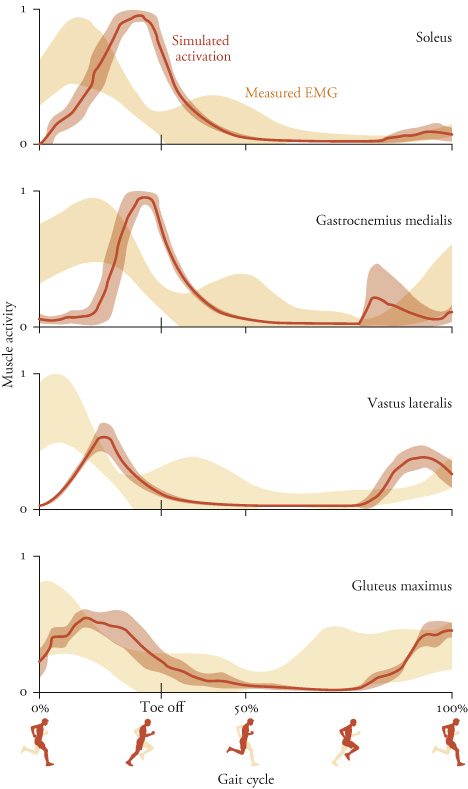
\includegraphics[width=0.8\linewidth]{chap10/10_11}
	\caption{以 5 米/秒的速度跑步时,4 块肌肉的模拟激活和肌电图记录。
		测量的肌电图与模拟激活之间约 75 毫秒的延迟与肌电图和力量产生之间的机电延迟一致\cite{hamner2013muscle}。。 \label{fig:10_11}}
\end{figure}


\textit{凯特$\cdot$斯蒂尔}在我实验室学习期间,研究了蹲伏步态如何影响膝关节负荷。
首先,她需要确定用她设计的典型步行模型计算出的负荷是否与全膝关节置换手术中植入人体膝关节的传感器测量的膝关节负荷相匹配。
最初进行这些比较时,我们发现模型预测的膝关节负荷大于用仪器植入物测量的负荷。
我们对模型进行了调整,直到获得足够准确的结果(图~\ref{fig:10_12})。
之后,我们确信可以用该模型研究蹲伏步态下的膝关节负荷。


\begin{figure}[!htb]
	\centering
	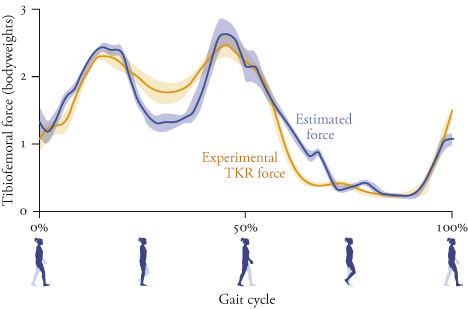
\includegraphics[width=0.8\linewidth]{chap10/10_12}
	\caption{胫股关节接触力在模拟中估算(蓝色),并通过器械\textit{全膝关节置换术}(橙色)测量。
		4 次试验的平均值±1个标准差\cite{steele2012compressive}。 \label{fig:10_12}}
\end{figure}


预测每块肌肉在运动过程中消耗多少代谢能量的能力是肌肉驱动模拟最强大的功能之一。
它之所以强大,是因为我们无法通过实验收集这些数据,但这对验证代谢成本的计算提出了挑战。
我们通常将模型中所有肌肉消耗的能量总和与通过间接量热法测得的能量消耗估计值进行比较(图~\ref{fig:10_13})。


\begin{figure}[!htb]
	\centering
	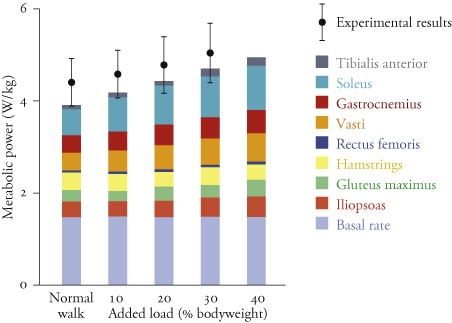
\includegraphics[width=0.8\linewidth]{chap10/10_13}
	\caption{正常步行和背负体重递增(最高可达受试者体重的 40\%)背包步行时的平均代谢功率。
		使用动态优化预测的总代谢功率(彩色条)与实验测量的总能量消耗(黑色;
		平均值±1 个标准差)呈现相似的趋势。
		“基础率”表示静息状态下的能量消耗\cite{dorn2015predictive}。 \label{fig:10_13}}
\end{figure}


在某些研究中,我们希望生成肌肉驱动的模拟,但实验数据很难甚至无法收集。
例如,我们可能希望评估数百种辅助设备设计,而无需构建昂贵的原型、招募测试对象或收集实验数据。
在这种情况下,我们可以先模拟无辅助行走,因为这类设备的实验数据很容易比较,只有在我们对模拟的预测有信心后,才开始研究辅助行走。


还必须执行软件测试,例如确认迭代算法收敛、满足数值积分公差以及遵循物理定律。确定计算模型是否准确表示底层数学模型的过程称为验证。
与确认(即询问“我是否求解了正确的方程?”)不同,验证过程涉及询问“我是否正确地求解了方程?”每次更改 OpenSim 软件时,我们都会执行数百次自动化软件测试,以确保不会在代码中引入错误。
这些测试至关重要,因为如果算法实现不正确,所有生成的模拟都将是错误的,研究的结论也会受到影响。
矛盾的是,大错误的问题最少,因为它们最容易被发现。
小错误可能最有害:它们可以产生看似合理的结果,因此可能被忽视。
通过以模块化方式设计软件可以促进验证,其中每个组件可以在对软件系统执行更高级别的测试之前进行独立测试(有时称为“单元测试”)。


计算关键输出对模型中具有较大不确定性的参数的敏感性通常很有用。
为了确保可靠性,研究结论必须对不确定输入的细微变化和任意的建模选择不敏感。
正如我们在第~\ref{chap:chap8}~章中指出的那样,所有模型都是错误的,但有些模型是有用的;
我们必须始终确保模拟结果是有用的,而不仅仅是错误的。
作为计算生物力学家,我们有责任确保已进行严格的软件验证,我们的模型和模拟已得到充分的确认,并且我们报告的结果对具有较大不确定性的参数不敏感。


\section{第四阶段:分析肌肉驱动的模拟}

为了从肌肉驱动的人体运动模拟中获得洞见,我们需要的不仅仅是经过适当验证的模拟。
最重要的是,我们必须提出一个模拟能够解答的问题(而实验无法更有效地解答这个问题)。
模拟计算了许多可以通过实验测量的量,这些量对于验证非常有用,但它们也提供了一些在实践中无法测量的量。
例如,通常无法测量肌肉在运动过程中产生的力量;
然而,在模拟中,肌肉力量可以通过肌肉收缩动力学模型计算出来,并且易于分析。
当结合关节运动学和肌肉路径的计算时,肌肉收缩动力学模型使我们能够估算肌腱应变,这是另一个难以在体内测量的量,并且在运动过程中能量的储存和释放中起着关键作用。


模拟可以让你执行强大的分析。例如,可以求解控制模型动力学的方程组,以确定每块肌肉的力量对加速模型重心(或任何其他点)的贡献。
这称为肌肉诱导加速度分析,它使用公式~\ref{eq:10_1}~计算由每块肌肉的力量作用于骨骼而引起的身体加速度。
该分析应用牛顿第二定律来确定每块肌肉的力量引起的加速度,这是在生物力学系统中建立因果关系的必要步骤。
请注意,这种分析是严格的回顾性的,不适合预测新的动作或肌肉补偿策略,例如,如果肌肉受伤的话。
正如我们将在第~\ref{chap:chap11}~章和第~\ref{chap:chap12}~章中看到的,肌肉诱导加速度分析可以揭示每块肌肉如何在行走时支撑身体的重量,以及如何在跑步时推动你前进。


模拟还能揭示因果关系,例如跟腱的柔顺性如何影响跑步的能量,并能预测假设情景的结果。
如果一个模型的力量加倍,它跑得会快一倍吗?
当肌肉无力时,它是否会采取跛行或蹲伏的步态?
模拟已经开始解答这些问题。



\section{用于创建肌肉驱动模拟的软件}

20 世纪 90 年代初,我和 Peter Loan 推出了交互式肌肉骨骼建模软件 SIMM。
该软件包允许用户创建、修改和分析多种肌肉骨骼结构的模型\cite{delp1995graphics}。
在接下来的十年里,研究人员创建了数十种人类和动物模型。
他们利用这些模型模拟行走、跑步、骑自行车、爬楼梯和病理步态,并研究手术重建的生物力学后果。
SIMM 促进了运动控制原理的探索,以及对运动病理患者的治疗。
我清楚地认识到,通过扩大用户群并允许用户更轻松地共享模型和模拟,我们可以加速研究。


2007 年,我和同事启动了 OpenSim 项目,这是一个扩展了 SIMM 功能的开源软件平台\cite{delp2007opensim}。
OpenSim 的功能涵盖 3 个方面。
首先,用户可以构建、操作和查询生物力学模型(图~\ref{fig:10_14})。
例如,骨骼标本已被用来构建南方古猿阿法种的手部模型,以研究这种灵长类动物是否具有足够的握力来制作某些石器\cite{domalain2017australopithecus}。
其次,OpenSim 可以实现一些实验难以完成的研究,例如研究如何利用肌腱弹性来提高跑步效率\cite{uchida2016stretching}。
第三,利用神经肌肉控制和动态模拟的原理,无需进行任何实验,OpenSim 就可以预测新的动作及其对新条件的适应性。
这种能力使我们对肌肉在预防踝关节损伤方面的作用有了更深入的了解\cite{demers2017preparatory}。


\begin{figure}[!htb]
	\centering
	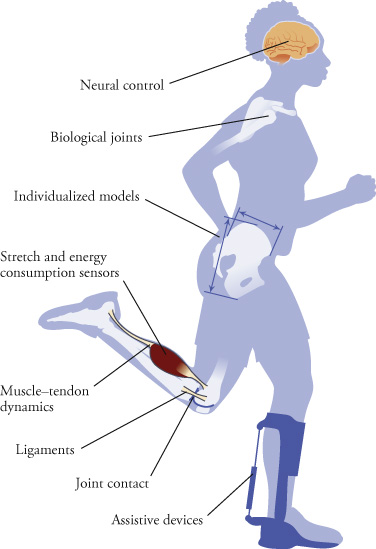
\includegraphics[width=0.65\linewidth]{chap10/10_14}
	\caption{OpenSim 可用于生成运动的正向动力学和逆向动力学模拟。
		该软件允许用户建模各种生物和机械系统,包括神经控制器、肌肉肌腱执行器和辅助设备\cite{seth2018opensim}。 \label{fig:10_14}}
\end{figure}


成千上万的生物力学家在 \href{http://simtk.org/}{simtk.org} 代码库上分享了 OpenSim 模型、模拟和计算工具。
我们创建这个代码库的目的是帮助研究人员复现、验证和扩展他人的研究成果。
我很高兴看到 OpenSim 社区不断发展壮大,日益多元化。
从跑鞋到骨科手术,最伟大的洞见很可能源于各个领域专家的通力合作。
OpenSim 为这种合作提供了一个平台。
在接下来的两章中,我们将分析在 OpenSim 中创建的模拟,以研究肌肉对人类行走和跑步的贡献,并了解这些模拟结果如何在现实世界中得到应用。
